\documentclass[16pt]{scrartcl}
\usepackage[T1] {fontenc}			%Fyrir íslenska sértafi
\usepackage[utf8] {inputenc}		%Fyrir Mac (íslenska sérstafi)
\usepackage[english] {babel}		%Fyrir íslenska sérstafi
\usepackage{pgf,tikz}
\usetikzlibrary{calc}
\usetikzlibrary{arrows}
\usepackage{wrapfig}
\usepackage{array}
% \usepackage{amsmath}
\usepackage{physics}
\usepackage{physunits}
% for numbering equations section wise
\usepackage[utf8]{inputenc}
\RequirePackage[l2tabu, orthodox]{nag}			% Nöldrar meira við villumeldingar
\usepackage[T1]{fontenc}						% Keyrir 8-bit font encoding sem kallast T1
\usepackage{microtype} 							% Ýmsar lagfæringar á stafabili og orðabili í build'i.
\usepackage{setspace} 							% Get notað \begin{doublespace} svæðið til að hafa tvöfalt línubil.
\usepackage[version=3]{mhchem} 					% Efnafræðipakkinn.
\usepackage[separate-uncertainty=true]{siunitx} % Læt siunitx pakkann skrifa óvissuna sem X \pm óvissa í stað sviga.
\usepackage{graphicx} 							% Required for the inclusion of images.
\usepackage{natbib} 							% Required to change bibliography style to APA.
\usepackage{amsmath} 							% Required for some math elements.
\usepackage[margin=3cm]{geometry} 				% Spássíur, breyta gildinu í hornklofanum.
\usepackage{epstopdf} 							% Til þess að geta buildað eps myndir í pdf'ið.
\usepackage{float} 								% Get meðhöndlað floats' eins og myndir með hástöfum [H].
\usepackage{caption} 							% Nauðsynlegur til þess að geta breytt mynda- og töflutextum.
\usepackage{subcaption}							% Nauðsynlegur til þess að gera myndatexta við fjölmyndir (e. subfigures)
% \usepackage{hyperref} 							% Nauðsynlegur til þess að breyta texta í klikkanlega hyperlinka.
\usepackage[colorlinks=true]{hyperref}
\newcommand*{\fullref}[1]{\hyperref[{#1}]{\autoref*{#1} \nameref*{#1}}}

\usepackage{marvosym}
\renewcommand{\arraystretch}{1,5}
\usepackage{amssymb}
\linespread{1.5}
\usepackage{xfrac}
\usepackage[nodayofweek,level]{datetime}

% custom numberin of equations
\numberwithin{equation}{section}
\newcommand\addtag{\refstepcounter{equation}\tag{\theequation}}

\usepackage{sectsty}
% this is, in fact, the default
% \sectionfont{\myfont}

% For using definitions, theorems and examples
\usepackage{amsthm}
\theoremstyle{plain}
\newtheorem{thm}{Theorem}[section] % reset theorem numbering for each chapter
\theoremstyle{definition}
% \newtheorem{defn}[thm]{Definition} % definition numbers are dependent on theorem numbers
% \newtheorem{exmp}[thm]{Example} % same for example numbers

\usepackage{incgraph}

\usepackage{blindtext}
\usepackage[most]{tcolorbox}
\newtcbtheorem[number within=section]{defn}{Definition}
{
    frame hidden,
    boxrule=0pt,
    left=0.2cm,right=0.2cm,top=0.2cm,
    toptitle=0.1cm+1pt,%        <-- I used your values here
    bottomtitle=-0.1cm+0.5em,% 
    colback=blue!2!white,
    colbacktitle={blue!5!white},
    coltitle={black},
    fontupper=\myfont,
    fonttitle={\slshape}
}
{def}

% for tikz
\usepackage{pgfplots}
\pgfplotsset{compat=1.11}

% for color or something
\usepackage{xcolor}

\title{Special Theory of Relativity}
\author{
    Jujhaar Singh
}
\date{}
\makeatletter

\usepackage{fancyhdr} % Headers and footers
\pagestyle{fancy} % All pages have headers and footers
\fancyhead{} % Blank out the default header
\fancyfoot{} % Blank out the default footer
\fancyhead[L]{\footnotesize\myfont \@title} % Custom header text
\fancyhead[R]{\footnotesize\myfont \@author} % Custom header text
\fancyfoot[C]{\footnotesize\thepage} % Custom footer text

\newcommand{\myfont}{\fontfamily{cmss}\selectfont}
\newcommand{\myfontb}[1]{\textbf{\myfont #1}}


\usepackage{setspace}
% \onehalfspacing
\setstretch{1}

\begin{document}
\pagenumbering{roman}

\incgraph[documentpaper][width=\paperwidth,height=\paperheight]{img/cover-SoS.jpg}

\pagebreak

\begin{titlepage}
    \centering
    {\scshape\LARGE Summer of Science 2021 \par}
    \vspace{1.5cm}
    
\includegraphics[width = 0.25\textwidth]
    {img/iitb_logo}\par
    \vspace{1cm}
    {\Huge \myfontb \@title \par}
    \vspace{3cm}
    {\Large\myfont
        \@author \par
        \large
        Mentor: Nabeel Ahmed
        \vfill
        {\large \@date \par}
    }\end{titlepage}

% \setcounter{page}{2}
\pagebreak
\thispagestyle{empty}
\tableofcontents
\pagebreak

\pagenumbering{arabic}
\setcounter{page}{1}


\section*{Introduction}
\addcontentsline{toc}{section}{Introduction}
This document contains a brief description of some of the key ideas of the Special Theory of Relativity. We follow the book ``Special Relativity and Classical Field Theory'' by Susskind and Friedman closely in its ideas and overall direction.

We shall first look at the effect on the coordinates on change of reference frame, which will be characterized by the Lorentz Transformation and find out how it arises and what it means physically. After this we will define the quantities that we will be using in our new system and strive to write laws of motion for them. 

This will finally read us to the famous expressions for energy that are predicted through this theory.

\pagebreak

\section{Reference Frames and the Lorentz Transformation}

The Special Theory of Relativity is mainly a theory about reference frames. We aim to find out that what remains the same between frames, and what changes, essentially, how physical quantities vary.

\subsection{Reference Frames}
\label{sec:RFs}

In physics, we deal with the motion and behavior of things that we observe. Of course, if we are to talk about objects in space, we would need some way to express physical parameters of said objects. For this purpose, we define Frames of Reference.

\begin{defn}{Reference Frames}{RFs}
    In space-time we say that a set of axis of x, y, z and along with that a reference for time is called a frame of reference.
    % \label{def:RFs}
\end{defn}

Having defined frames of reference, we are ready to define a very special sub-category that is an integral part of the rest of our study.

\begin{defn}{Intertial Reference Frames}{IRFs}
    We define inertial frames of reference as those in which particles, on which no external force is acting, move in a straight line with constant speed. For a frame to be inertial, it must have zero acceleration.
    % \label{def:IRFs}
\end{defn}

Ones of the aims for both Einstein and Newton was to find a set of laws that can accurately predict the motion of particles, and are applicable, without modification, in all inertial reference frames. This led to Einstein figuring out that if the laws remain the same, then the speed of light should also be the same in all frames of reference and for all observers.

\subsection*{Units and Dimensions}

In the units we generally use, the SI system, a velocity of magnitude 1 relates to an object moving one meter in one second. This also has the dimension of length over time. We shall call these ``conventional or common units''.

Since a lot of Relativistic physics deals with the speed of light, we would like to introduce a new set of units such that they have an inherent connection to the speed of light. In fact, this is a great way to reduce the complexity of many of the expressions we deal with. We define our new units in such a way that a velocity of magnitude 1 will be equal to the speed of light in conventional units. We will also choose it in such a way that this quantity is dimensionless. We will refer to these units as ``Relativistic units'' for the rest of the document.

\subsubsection*{Converting to and fro}

Later in the document, formulas may be represented in either set of units. To convert from one to the other, we simply use dimensional analysis and divide or multiply some power of $c$, the speed of light, to each term such that the eqaution becomes dimensionally correct.

\subsection{Problem with Newtonian Frames of Reference}

We consider a simple one dimensional system with the x axis positive on the right hand side and negative on the left hand side. For an inertial frame A, say we have another frame B moving to the right with a speed of v. We can write down a simple equation to describe its motion.

\begin{equation}
    x = vt
    % \label{eq:1.1}
\end{equation}

Now, for the stationary frame, A, we can say that a light ray moving to the right would have the following equation to describe its motion.

\begin{equation}
    x = ct
    % \label{eq:1.2}
\end{equation}

Looking at the same ray of light in the frame B, we get the following equation.

\begin{equation}
    x = (c - v)t
    % \label{eq:1.3}
\end{equation}

This makes sense to us by the common knowledge that we have of Newtonian physics. Looking closely at the equations, we find that the speed of light seems to be different in both. But recall what we said towards the end of \fullref{sec:RFs}. If we examine that assumption, then we see that since the laws of physics remain the same in all inertial frames, the speed of light, which is a direct result of those laws, should also remain the same in all reference frames. Clearly, that is not followed in Newtonian reference frames as shown above.

We will see that the principle assumption of Newtonian reference frames, that is, that the time in all frames moves at the same rate, is challenged by the theory of relativity. In fact, deleting that assumption is the only way to make the laws of physics consistent, as we will see later.

\subsection{Transformations in Relativistic Reference Frames}

\subsubsection{Space-time}

We will generally represent space-time with two axes, that is, one for time and one for distance, since we will consider a single dimension of space for simplicity. Space-time plots will generally look something like this \nameref{fig:space-time-basic}.

\begin{figure}
    \centering
    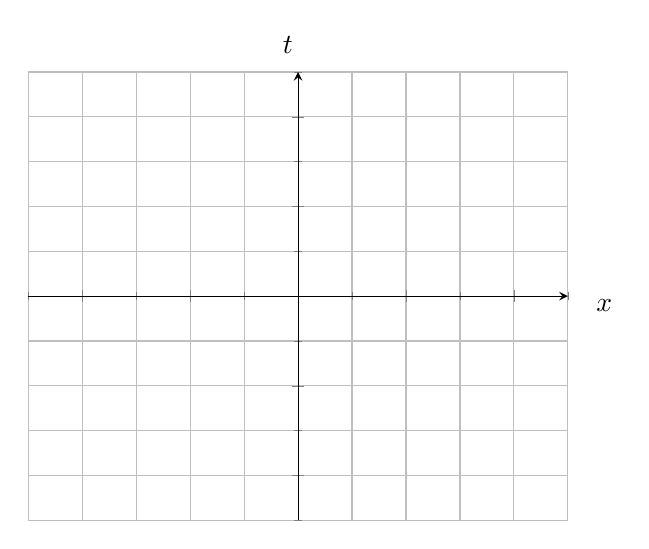
\begin{tikzpicture}
        \begin{axis}[grid=both,ymin=-5,ymax=5,xmax=5,xmin=-5,xticklabel=\empty, yticklabel=\empty,
                minor tick num=1,axis lines = middle,xlabel=$x$,ylabel=$t$,label style =
                    {at={(ticklabel cs:1.1)}}]
        \end{axis}
    \end{tikzpicture}
    \caption{basic space-time plot}
    \label{fig:space-time-basic}
\end{figure}

A more formal definition can also be given.

\begin{defn}{Space-time}{space-time}
    The concepts of time and three-dimensional space regarded as fused in a four-dimensional continuum.
    % \label{def:space-time}
\end{defn}

We will see that this same definition can be used in a simplified form for just the $x$ axis. In this case, it would be the time dimension plus one dimensional space, giving us a two dimensional space representing both space and time.

\begin{defn}{Space-time events}{event}
    We define a space-time event as one which has a time coordinate as well as space coordinates. In an n-dimensional space, a space-time event would look like $(t,x_1,x_2 \dots x_n)$ where $x_1,x_2 \dots x_n$ represent n space coordinates.
    % \label{def:event}
\end{defn}

\subsubsection{Synchronizing}

To be able to talk about space-time events in different reference frames, we would need some sense of what "synchronous" events would mean. One simple definition that can be used is given below.

\begin{defn}{Synchrony}{sync}
    Say we have 3 objects, A, B and C, moving through space in such a way that B is always at the midpoint of A and C. Let their paths be defined as $a(t)$, $b(t)$ and $c(t)$ respectively. Now, a light ray is sent from A to B at $t_1$ and another is sent from C to B at $t_2$. If these two reach B at the same time, then we say that the space-time events ($t_1, a(t_1)$) and ($t_2, c(t_2)$) synchronous.
    % \label{def:sync}
\end{defn}

The meaning of synchronous changes according to the observer and his frame of reference. With respect to space-time plots, two points that are synchronous should have the same time coordinate with respect to the axes of that frame to be considered synchronous. This of course only applies in the frame which we were considering, thus they may happen at different times in a different frame of reference.

\subsubsection{The Lorentz Transformation}

We know that any reference frame can be represented by the time and space axes. For yourself, your distance and time axes are perpendicular to each other. We take the time axis along the vertical and x(distance) along the horizontal.

If we would like to find how the axes looks for an observer who is moving relative to us, we can use the notion of \nameref{def:event} and their \nameref{def:sync} to find the position of their axes.

Using the above discussed concepts of the synchrony of events, constancy of speed of light in all frames, and a few other concepts and manipulations, we arrive at the Lorentz Transformation. This transformation dictates how the space and time axes look for a person in a different inertial frame of reference from our resting frame. 
\begin{gather}
    t' = \frac{t-vx/c^2}{\sqrt{1-v^2/c^2}} \\
    x' = \frac{x-vt}{\sqrt{1-v^2/c^2}} \\
    y' = y\\
    z' = z
    \label{eq:lorentz}
\end{gather}

This kind of a transformation is also referred to as a boost along the x direction.

\subsection{Length Contraction and Time Dilation}

\subsubsection*{Length Contraction}
\hspace{\fill}
Say I am stationary and standing at the origin. I have a meter stick in my hand, which extends from the origin, $O$, to the point $Q$ in my frame of reference. Now suppose a person A, who is moving towards the positive x direction at a speed $v$, moves past me. At the point that he crosses me, if he were to measure my meter stick with his set of axes, will the meter stick have a length of $1m$? (assume the time that he crosses me is $t=0$ in both our clocks)

In fact, it will not, for him the stick will appear shorter. This is the phenomena of length contraction and it is represented in \autoref{fig:length-contraction}($t,x$are my axes and $t',x'$ represent his). For person A, points $O$ and $Q$ are not simultaneous since they do not lie on the $x'$ axis. For him, the stick is along $OP$ when he crosses me. That is, the length of the stick for him is the length along the axis $x'$ from the point $O$ to the point $P$. 

Something looks a little suspicious here. Doesn't $OP$ look longer than $OQ$? Then how come the length he sees is shorter? This is because the ticks along the $x'$ axis have a different spacing than the ticks along the $x$ axis. It is a simple consequence of the Lorentz Transformation and you can easily verify this. 

Thus, the length of the meter stick measured by person A will be given by \autoref{eq:length-formula} \footnote{note that we are working in relativistic units}.

\begin{equation}
    \sqrt{1-v^2}
    \label{eq:length-formula}
\end{equation}


\hspace{\fill}
\begin{figure}
    \centering
    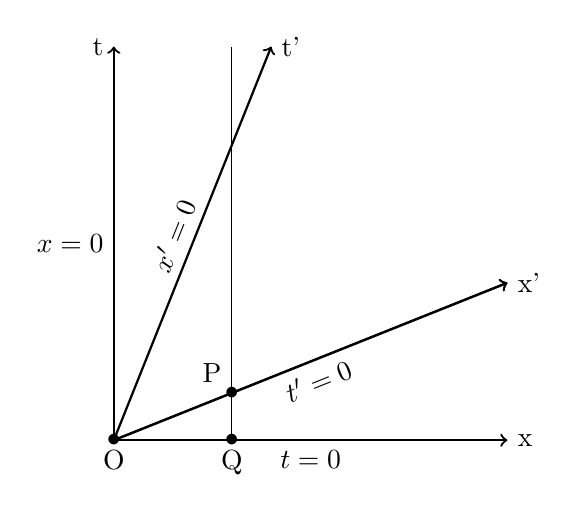
\begin{tikzpicture}[thick]
        \draw[->] (0,0) -- (0,5) node[left] {t} node[midway,left] {$x=0$};
        \draw[->] (0,0) -- (5,0) node[right] {x} node[midway,below] {$t=0$};
        \draw[->] (0,0) -- (2,5) node[right] {t'} node[midway,sloped,above] {$x'=0$};
        \draw[->] (0,0) -- (5,2) node[right] {x'} node[midway,sloped,below] {$t'=0$};
        \draw[->] (0,0) -- (5,2);
        \draw (1.5,0.6) node{$\bullet$} node[above left] {P};
        \draw (1.5,0) node{$\bullet$} node[below] {Q};
        \draw (0,0) node{$\bullet$} node[below] {O};
        \draw[thin,-] (1.5,0) -- (1.5,5);
    \end{tikzpicture}
    \caption{length contraction}
    \label{fig:length-contraction}
\end{figure}

\subsubsection*{Time dilation}
% \hspace{\fill}

Time dilation works in a similar way. Say I am now moving with a clock in my hand while you are standing still. I started the clock at $x=0$ and at point Q I see that the clock reads time $t'=1$. The question now is, what is the time on your clock at this point? This situation is represented in \autoref{fig:time-dilation}

Notice that the surface $PQ$ is what you call synchronous. Using the Lorentz Transformation once again, you can obtain the expression in \autoref{eq:time-formula} \footnote{again, we are working in relativistic units} for time passed in the stationary reference frame.

\begin{equation}
    \frac{1}{\sqrt{1-v^2}}
    \label{eq:time-formula}
\end{equation}

% \vfill

\begin{figure}
    \centering
    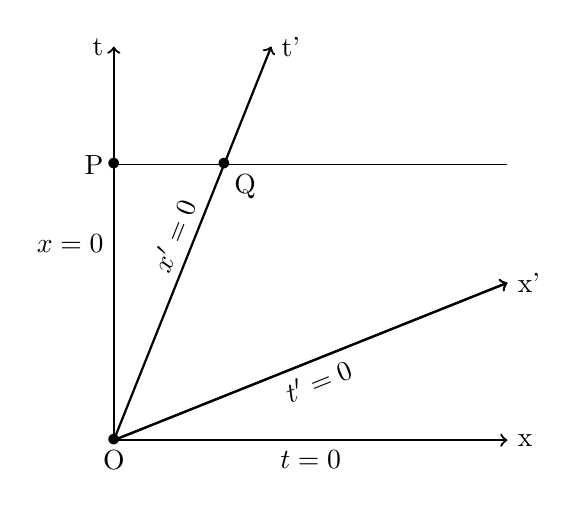
\begin{tikzpicture}[thick]
        \draw[->] (0,0) -- (0,5) node[left] {t} node[midway,left] {$x=0$};
        \draw[->] (0,0) -- (5,0) node[right] {x} node[midway,below] {$t=0$};
        \draw[->] (0,0) -- (2,5) node[right] {t'} node[midway,sloped,above] {$x'=0$};
        \draw[->] (0,0) -- (5,2) node[right] {x'} node[midway,sloped,below] {$t'=0$};
        \draw[->] (0,0) -- (5,2);
        \draw (0,3.5) node{$\bullet$} node[left] {P};
        \draw (1.4,3.5) node{$\bullet$} node[below right] {Q};
        \draw (0,0) node{$\bullet$} node[below] {O};
        \draw[thin,-] (0,3.5) -- (5,3.5);
    \end{tikzpicture}
    \caption{time dilation}
    \label{fig:time-dilation}
\end{figure}

\subsection{Minkowski Space}

The space-time diagrams we draw exist in what is called Minkowski Space. This is similar to our notion of cartesian space which contains the $x$, $y$, and $z$ dimensions. In Minkowski Space, instead of having just the three spatial dimensions, we also have time represented along another direction. For obvious reasons we cannot really represent, or even imagine, a Minkowski space in 3 space dimensions and 1 time dimension since we run out of direction to orient our axes in. Thus we generally use diagram draw for 2 spatial dimensions and 1 time dimension. 

\subsubsection*{Invariants}

The concept of invariants is very widely used in physics, but you may not have pondered on it too much. This is because in our box of Newtonian mechanics, we have a very intuitive invariant. Time. 

In Relativistic terms however, time is clearly not an invariant as we have seen above. From frame to frame we have different measurements of time and all observers do not agree on it. It can be found with some algebra that the invariant in Relativistic cases is something that we call ``proper time''. It's symbol is $\tau$.

\begin{equation}
    \tau^2 = t^2 - x^2 - y^2 - z^2
    \label{eq:propertime}
\end{equation}

This quantity, just like time in the Newtonian world, is constant over all frames of reference, for all observers and through any Lorentz transformation. Thus it is an invariant. 

Even though right now it may not mean much to you, $\tau^2$ does hold physical and experimental significance. Say we are sitting at the origin and someone, person A, crosses us. When $t$ seconds pass in our frame of reference person A is at $x_0$ in our frame. Say at this point, $t'$ seconds have passed in person A's frame. Since the proper time of the event at the location of person A must be same in both the frame, we get the following.

\begin{gather}
    \tau'^2 = t'^2 - x'^2 \text{ but } x'=0 \text{ for person A} \\
    % \text{but $x'=0$ for person A in his frame by defintion}\\
    \implies \tau'^2 = t'^2\\
    \text{also, } \tau^2 = t^2 - x^2\\
    \implies t'^2 = t^2 - x^2
    \label{eq:proper-time-significance}
\end{gather}

We also define the space-time interval as the following. Of course this quantity too is an invariant.

\begin{equation}
    s^2 = x^2 + y^2 + z^2 - t^2 = - \tau^2
    \label{eq:spacetime-interval}
\end{equation}



\subsubsection*{The Light Cone and Space-time Separations}

Imagine a two dimensional plane on which you represent x and y. Now add a third line perpendicular to the plane in order to represent time. This now forms a Minkowski Space of two space dimensions and one time dimension. 

Now imagine how you would represent a light "ring" emitting from the point $x = 0$ and $y = 0$ at time $t = 0$. This is the analog of a point source of light in two dimensions. Notice that it would form a cone in the Minkowski Space. This is illustrated in \fullref{fig:light-cone}.

The equation of this cone is given by $x^2 + y^2 + z^2 = c^2 t^2$ as you might have guessed. But in relativistic coordinates of course this simplifies to $x^2 + y^2 + z^2 = t^2$.

\begin{figure}
    \centering
    \begin{tikzpicture}
        \draw[->] (5,0) -- (5,10) node[left] {t};
        \draw[->] (8,7.5) -- (2,2.5) node[below] {y};
        \draw[->] (0,5) -- (10, 5) node[right] {x};

        \draw[dashed] (2,1) arc (170:10:3cm and 0.4cm)coordinate[pos=0] (a);
        \draw (2,1) arc (-170:-10:3cm and 0.4cm)coordinate (b);
        \draw (a) -- ([yshift=4cm]$(a)!0.5!(b)$) -- (b);

        \draw[dashed] (2,9) arc (170:10:3cm and 0.4cm)coordinate[pos=0] (c);
        \draw (2,9) arc (-170:-10:3cm and 0.4cm)coordinate (d);
        \draw (c) -- ([yshift=-4cm]$(c)!0.5!(d)$) -- (d);
    \end{tikzpicture}
    \caption{Light Cone}
    \label{fig:light-cone}
\end{figure}

Now we define a ``Time-like'' event.

\begin{defn}{Time-like event}{timelike}
    When an event lies within the light cone, ie $x^2+y^2+z^2 < t^2$, then we say that the separation is ``time-like'' with respect to the origin. The time separation is larger than the space separation from the origin for these events.
\end{defn}

For a time-like event, we can always find a frame such that the two events occur at the same spatial location in that frame but at different times. We also say that there is no frame in which these two events occur simultaneously.

Similarly we define ``Space-like'' events.

\begin{defn}{Space-like event}{spacelike}
    When an event lies outside the light cone, ie $x^2+y^2+z^2 > t^2$, then we say that the separation is ``Space-like'' with respect to the origin. The space separation is larger than the time separation from the origin for these events.
\end{defn}

For a space-like event, we can always find a reference frame such that the two events occur simultaneously but at different spatial locations in that frame. We cannot, however, find a reference frame in which both the events occur at the same location in space.

Finally we also define ``light-like'' intervals.

\begin{defn}{Light-like Events}{lightlike}
    When an event lies on the light cone, ie $x^2+y^2+z^2 = t^2$, then we say that the separation is ``light-like'' with respect to the origin. The time separation is equal to the space separation from the origin for these events.
\end{defn}

If two events are light-like it means that there is a possibility of a light ray going from one and reaching the other.

\section{4-Vectors and Velocities}

\subsection{4-Vectors}

\begin{defn}{4-Vector}{4vec}
    If a vector with 4 coordinates transforms according to the rules of the Lorentz transform then we call it a 4-Vector.
\end{defn}

A 4-Vector can be used to define an event in a space-time diagram. It consists of one time coordinate and three space coordinates. The first coordinate is time and the next three are space coordinates, say $x$, $y$, and $z$.

\subsubsection*{Some notation}

We may use the following notation to represent a 4-Vector.

\begin{equation}
    (X^0, X^1, X^2, X^3)
    \label{eq:4-vector}
\end{equation}

The above representation implies the following.
\begin{gather}
    t = X^0\\
    x = X^1\\
    y = X^2\\
    z = X^3
    \label{eq:4-vector-comps}
\end{gather}

We will also use $X^i$ to talk about only the space components and $X^\mu$ to talk about all four components together.
\begin{gather}
    X^i \implies (X^1, X^2, X^3)\\
    X^\mu \implies (X^0, X^1, X^2, X^3)
    \label{eq:4-vec-notation}
\end{gather}

\subsection{4-Velocity}

This is just the counterpart to velocity for 4-Vectors. One major difference from normal velocity is that here we consider variation over proper time instead of time. This is convenient because proper time is an invariant too. Thus we define 4-Velocity as the following.

\begin{gather}
    U^0 = \dv{X^0}{\tau} = \dv{t}{\tau}\\
    U^1 = \dv{X^1}{\tau} = \dv{x}{\tau}\\
    U^2 = \dv{X^2}{\tau} = \dv{y}{\tau}\\
    U^3 = \dv{X^3}{\tau} = \dv{z}{\tau}
    \label{eq:4-velocity}
\end{gather}

\subsection{More on 4-Velocity}

There is an interesting relation between normal velocity and 4-Velocity. We will denote the 4-velocity using $U^i$ and the normal velocity using $V^i$.
\begin{gather}
    U^0 = \frac{1}{\sqrt{1 - v^2}}\\
    U^i = \frac{V^i}{\sqrt{1 - v^2}}
    \label{4vel-normalvel}
\end{gather}

Another property of 4-velocity is that its components are connected by an invariant. This is analogous to how proper time is an invariant for position represented by 4-vectors. This invariant quantity is equal to 1 and further implies that only any three components of the 4-velocity are independent and the fourth is a dependent.

\begin{equation}
    (U^0)^2 - (U^1)^2 - (U^2)^2 - (U^3)^2 = 1
    \label{eq:4vel-invariant}
\end{equation}

\section{Relativistic Laws of Motion}

\subsection{Principle of Least action, Lagrangian and Hamiltonian}

This principle states that a process will happen in such a way that a certain defined quantity called action is minimized over the process. The action is the integral of Lagrangian over time during the process. Based on the system we define the Lagrangian.

In a simple Newtonian system where no forces act on a particle, the Lagrangian is simply the kinetic energy of the particle.

The Hamiltonian of a system is generally representative of the total energy of a system and a simple relation exists between the Hamiltonian and the Lagrangian given by the following.

\begin{equation}
    H = \sum_i \dot X^i P^i - \mathcal{L}
    \label{eq:ham-lag}
\end{equation}

Here $P^i$ represent the components of the particle's momentum.

\subsection{Relativistic Action}

In relativity, we define the action as the following.

\begin{equation}
    Action = -m \int_a^b d\tau = -m \int_a^b \sqrt{1-v^2} dt
    \label{eq:rel-action}
\end{equation}

This leads us to defining the Lagrangian for relativistic systems.

\begin{equation}
    \mathcal{L} = -m \sqrt{1 - v^2} = -m \sqrt{1 - (\dot X^i)^2} 
    \label{eq:rel-lagrangian}
\end{equation}

If we rewrite this expression in terms of conventional units we obtain the following.

\begin{equation}
    \mathcal{L} = -mc^2 \sqrt{1 - \frac{v^2}{c^2}}
    \label{eq:rel-lag-conventional}
\end{equation}

\subsection{Relativistic Momentum}

In Lagrangian mechanics we define the moment as the derivative of the Lagrangian $\mathcal{L}$ with respect to $\dot X$. So now we try to extend this notion to try and define relativistic momentum.

\begin{equation}
    P^i = \pdv{\mathcal{L}}{\dot X^i}
    \label{eq:rel-momentum}
\end{equation}

This gives us the following.

\begin{equation}
    P^i = \frac{mV^i}{\sqrt{1- \frac{v^2}{c^2}}} = mU^i = m \dv{X^i}{d\tau}
    \label{eq:rel-momentum-2}
\end{equation}

\subsection{Relativistic Energy}

To define energy, we take help of \eqref{eq:ham-lag} and try to extend its definition beyond what it is meant for. This gives us the following.

\begin{equation}
    H = \frac{m}{\sqrt{1-v^2}}
    \label{eq:rel-energy}
\end{equation}

Interestingly this is the ``zeroth'' component of our relativistic momentum, given by \eqref{eq:mom-zeroth}.

\begin{equation}
    P^0 = mU^0 = H = \frac{m}{\sqrt{1-v^2}} 
    \label{eq:mom-zeroth}
\end{equation}
 
This $P^0$ with our previously discovered $P^i$ gives us a 4-vector! The implications of this are that the energy and the momentum of a particle get mixed up during a lorentz transform. This is why
we may find the particle having a momentum in one frame but not the other or another particle having energy in one frame but not the other. 

Another important take away is that our previous notion of conservation of momentum now turns into the conservation of the 4-momentum instead.

This energy written in conventional units gives us \eqref{eq:rel-energy-conventional}

\begin{equation}
    H = \frac{mc^2}{\sqrt{1-\frac{v^2}{c^2}}}
    \label{eq:rel-energy-conventional}
\end{equation}

\subsubsection*{Slow Particles and $mc^2$}

Now imagine the case of a particle for which $v$ is far less than the speed of light. This gives us the following relation using approximations.
\begin{equation}
    H = \frac{mc^2}{\sqrt{1-\frac{v^2}{c^2}}} = mc^2 \left(1 + \frac{v^2}{2c^2} \right) = \frac{1}{2} mv^2 + mc^2
    \label{eq:rel-energy-slow}
\end{equation}

This tells us that when the particle is at rest, ie $v=0$, the energy of the particle will be given by the famous Einstein equation \eqref{eq:einstein}.

\begin{equation}
    E = mc^2
    \label{eq:einstein}
\end{equation}

This quantity represents the energy of the body in a frame where it is at rest. This equation also famously represents mass-energy equality and is thus an equation of utmost importance.

\subsubsection*{Relation between energy, momentum and mass}

Now recall the relation \eqref{eq:4vel-invariant}. This relation defines the invariant quantity for 4-velocity. As it turns out, we can use it to arrive at a relation between the above mentioned quantities. We simply multiply the whole equation with $m^2$ and then substitute various quantities based on the definitions given by us. We finally obtain:

\begin{equation}
    E = \sqrt{P^2+m^2}
    \label{eq:epm-relation}
\end{equation}

Rewriting this in conventional units gives us a less famous but equally important relation. 

\begin{equation}
    E = \sqrt{P^2c^2+m^2c^4}
    \label{eq:epm-relation-conventional}
\end{equation}

This holds significance because it gives us a complete description of the energy term. It is valid in all cases including for particles with no mass, no momentum, etc.

\section{Conclusion}

With this we get to the end of this paper. While it has been short, I certainly hope that it was of value to the reader. One major objective was to explain what the whole fuss about the mystical relation between energy and mass is. I hope that this paper has been adequate to convey the relevance of the same.

\end{document}

